\documentclass{article}

\usepackage{geometry}
\usepackage{amsmath}
\usepackage{graphicx, eso-pic}
\usepackage{listings}
\usepackage{hyperref}
\usepackage{multicol}
\usepackage{fancyhdr}
\pagestyle{fancy}
\fancyhf{}
\hypersetup{ colorlinks=true, linkcolor=black, filecolor=magenta, urlcolor=cyan}
\geometry{ a4paper, total={170mm,257mm}, top=40mm, right=20mm, bottom=20mm, left=20mm}
\setlength{\parindent}{0pt}
\setlength{\parskip}{0.3em}
\renewcommand{\headrulewidth}{0pt}
\rfoot{\thepage}
\lfoot{Seleksi IEEEXtreme 15.0 ITB}
\lstset{
    basicstyle=\ttfamily\small,
    columns=fixed,
    extendedchars=true,
    breaklines=true,
    tabsize=2,
    prebreak=\raisebox{0ex}[0ex][0ex]{\ensuremath{\hookleftarrow}},
    frame=none,
    showtabs=false,
    showspaces=false,
    showstringspaces=false,
    prebreak={},
    keywordstyle=\color[rgb]{0.627,0.126,0.941},
    commentstyle=\color[rgb]{0.133,0.545,0.133},
    stringstyle=\color[rgb]{01,0,0},
    captionpos=t,
    escapeinside={(\%}{\%)}
}

\begin{document}

\begin{center}
    \section*{Jajargenjang} % ganti judul soal

    \begin{tabular}{ | c c | }
        \hline
        Batas Waktu  & 2 s \\    % jangan lupa ganti time limit
        Batas Memori & 256 MB \\  % jangan lupa ganti memory limit
        \hline
    \end{tabular}
\end{center}

\subsection*{Deskripsi}
Pada update 4.20, Ish’kafel mendapatkan buff pada ultimate skillnya, "Wall of Replica". Dengan skill ini, Ish’kafel dapat meletakkan tembok berupa garis lurus dengan panjang tak hingga pada bidang 2 dimensi. Garis yang diletakkan harus memiliki persamaan garis $a x + b y = c$, serta Ish’kafel hanya dapat menaruh maksimal $10^5$ tembok. Untuk memperangkap musuhnya, Ish’kafel ingin membentuk tepat $K$ buah jajargenjang berluas tak nol yang disusun dari tepat 4 buah tembok dari $N$ tembok yang dia letakkan. Sebuah bangun dikatakan sebagai jajargenjang jika memiliki 4 sisi dan 2 pasang sisi yang berhadapan saling sejajar. Bantulah Ish’kafel menyelesaikan masalah tersebut.

\subsection*{Format Masukan}
Input hanya berisi satu baris yakni bilangan $1 \leq K \leq 10^9$.

\subsection*{Format Keluaran}
Baris pertama berisi banyaknya garis $1 \leq N \leq 10^5$.

$N$ baris berikutnya berisi 3 bilangan bulat $-100 \leq a_i, b_i, c_i \leq 100$, yang menandakan persamaan garis ke-$i$ ialah $a_i x + b_i y = c_i$. Tidak boleh ada 2 garis berbeda $1 \leq i < j \leq N$ sehingga kedua garis bersinggungan.

Keluarkan satu saja dari banyak jawaban yang mungkin. Bila tidak mungkin cukup keluarkan $1$ baris berisi $-1$.

\begin{multicols}{2}
\subsection*{Contoh Masukan 1}
\begin{lstlisting}
2

\end{lstlisting}
\columnbreak
\subsection*{Contoh Keluaran 1}
\begin{lstlisting}
-1

\end{lstlisting}
\vfill
\end{multicols}

\begin{multicols}{2}
\subsection*{Contoh Masukan 2}
\begin{lstlisting}
3
\end{lstlisting}
\null
\null
\null
\null
\null
\null
\null
\null
\columnbreak
\subsection*{Contoh Keluaran 2}
\begin{lstlisting}
5
1 1 -1
1 1 0
1 1 1
-1 1 -1
-1 1 1
\end{lstlisting}
\vfill
\null
\end{multicols}

\subsection*{Penjelasan}
\begin{center}
    \fbox{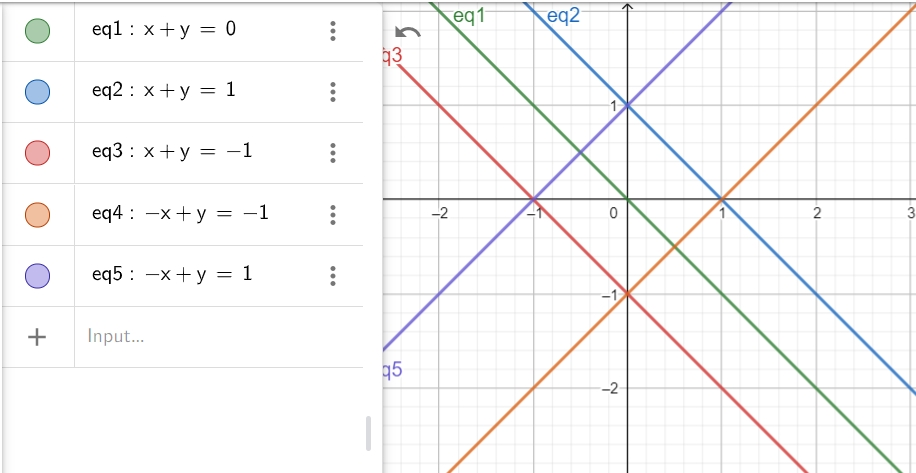
\includegraphics[scale=0.4]{jajargenjang.jpg}}
\end{center}
Tiga jajargenjang yang dihasilkan dibentuk oleh $(eq1, eq2, eq4, eq5), (eq2, eq3, eq4, eq5), (eq3, eq1, eq4, eq5)$

\end{document}